\section{Modello di sviluppo} \label{modello di sviluppo}

    \subsection{Ciclo di vita del software}

        Considerate le modalità di interazione e le richieste della \glossaryItem{Proponente}, il team ha deciso di adottare il
        \glossaryItem{modello incrementale}.

        Questo modello, infatti, consiste nella realizzazione incrementale del prodotto tramite l'iterazione di fasi
        composte da attività di progettazione in dettaglio e di realizzazione.

        \begin{figure}[htbp]
            \centering
            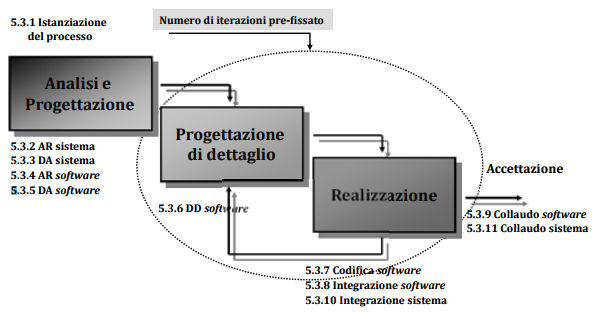
\includegraphics[scale=0.75]{./img/ModelloIncrementale.png}
            \caption[Immagine del modello di sviluppo incrementale]{Schema del modello incrementale secondo ISO 12207:1995}
        \end{figure}

        Ne consegue la possibilità di pianificare fasi atte alla realizzazione del \glossaryItem{Proof of Concept} e
        della baseline architetturale per adempire ai rispettivi obblighi imposti da Technology Baseline e Product Baseline.
        In particolare, il rendere il Proof of Concept parte integrante del prodotto comporterà un risparmio in termini
        di tempo e denaro.

        Ulteriori vantaggi sono i seguenti:

        \begin{itemize}
            \item L'istanziazione di gran parte dei processi e delle relative attività avviene fin dalle fasi iniziali.
            Ciò facilita la valutazione e la raffinazione tramite norme, anticipando l'insorgere di eventuali problemi,
            come quelli causati da \glossaryItem{big-bang integration};
            \item I requisiti possono essere etichettati con dei livelli di priorità. Tenendo conto di questo sarà
            possibile anticipare lo sviluppo dei requisiti obbligatori già dalle fasi iniziali. Le attività di verifica
            negli incrementi successivi solidificheranno questi requisiti;
            \item Viene minimizzato il rischio di non soddisfacimento dei requisiti fondamentali grazie alla possibilità
            di feedback anticipato da parte della Proponente.
        \end{itemize}
        
	\subsubsection{Incrementi del progetto}
	Nella pianificazione di un modello incrementale è importante fissare un limite superiore al numero di incrementi e di conseguenza
	il gruppo ha deciso di fissare questo limite a 10 incrementi. Questo permetterà di avere
	milestone di riferimento rispetto al progresso complessivo pianificato e di poter individuare e rimediare a problemi 			insorti in 	maniera preventiva.\\
	Ad ogni milestone sarà associata una baseline alla quale, a sua volta, è associato un incremento significativo del prodotto.
	Il primo incremento si baserà sul lavoro svolto nel Proof of Concept che implementerà i requisiti più significativi del progetto
	al fine di ottenere un'applicazione funzionante quanto prima.\\
	Con gli incrementi successivi verranno implementati i sottoinsiemi di requisiti
	mancanti, scelti secondo criteri di importanza, assegnando una priorità più alta per quelli obbligatori e con più alto grado di
	dipendenza. Questa scelta permetterà i seguenti vantaggi:
	\begin{itemize}
		\item I requisiti con priorità maggiore attraverseranno più fasi di verifica risultando dunque più raffinati rispetto ai requisiti 				meno significativi;
		\item L'integrazione di singoli sottogruppi di requisiti, con quanto realizzato fino a quel momento, eviterà il problema del big-bang 		integration;
		\item La scelta dei requisiti da implementare potrà essere fatta in modo da massimizzare l’utilizzo delle risorse disponibili e 				parallelizzarne lo sviluppo, avendo garanzie di efficienza ed efficacia.
	\end{itemize}
	Per gli incrementi successivi a quelli del PoC è stato associato un incremento per ogni realizzazione di componente. Dopo aver analizzato 	i requisiti, il gruppo ha pianificato la realizzazione di 9 componenti e da questo numero deriva la scelta di avere massimo 10 					incrementi.